\documentclass[a4paper,12pt]{article}

% Packages
\usepackage[utf8]{inputenc}  % Special characters
\usepackage{amsmath, amssymb} % Mathematical symbols
\usepackage{graphicx} % Including graphics
\usepackage{caption} % Captions for figures
\usepackage{geometry} % Adjusting page margins
\geometry{a4paper, left=2.5cm, right=2.5cm, top=2.5cm, bottom=2.5cm}

\begin{document}
    
    \title{Grid Synchronisation}
    \author{Simon Peter}
    \date{\today}
    \maketitle
    
\begin{abstract}
Dieses Repository enthält eine einfach zu implementierende Grid-Synchronisationsschaltung.
\end{abstract}


\section{Einleitung}
Das Repository enthält die Hardware, bestehend aus einem KiCad-Schaltplan und einem zugehörigen Layoutentwurf. Außerdem ist die Software für einen STM32 Nucleo H755 enthalten.


\section{Hardware}
Nachfolgend wird eine Schaltung vorgestellt, mit der die Netzfrequenz isoliert abgegriffen und der aktuelle Netzzeitpunkt softwareseitig ermittelt werden kann. Die Schaltung besteht aus zwei Komparatoren, welche die Höhe der Netzspannung vergleichen und so auf den Nulldurchgang schließen. Nachteilig an Komparatoren ist die Notwendigkeit einer Spannungsversorgung. Deshalb werden Opto-Emulatoren vom Typ ISOM8710 verwendet, die sich ähnlich wie Optokoppler verhalten. Opto-Emulatoren haben gegenüber Optokopplern jedoch verbesserte Parameter, wie beispielsweise eine höhere Störfestigkeit gegenüber schnellen Gleichtaktspannungen (engl. \textit{High Common Mode Transient Immunity} CMTI).

\begin{figure}[htb]
    \footnotesize
    \centering
    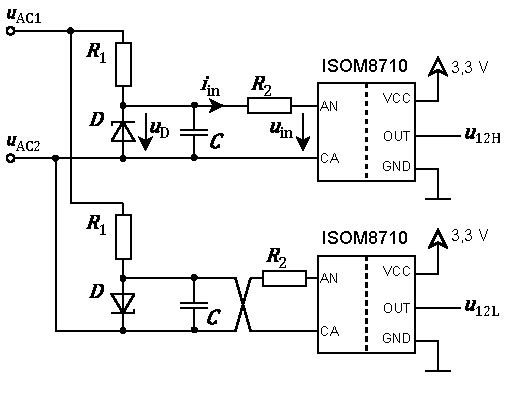
\includegraphics[width=0.65\linewidth]{HwGridSync}
    \caption{Isolierte Erfassung des Netznulldurchgangs um die Netzfrequenz sowie softwareseitig den Netzzeitpunk zu ermitteln.}	
    \label{fig:HwGridSync}
\end{figure}

Der erste Opto-Emulator (Abbildung~\ref{fig:HwGridSync} oben) soll schalten, wenn in der positiven Halbwelle die Eingangsspannung $u_\text{in}$ ausreichend hoch ist. In der anderen Halbwelle darf er nicht schalten. Mit einer Z-Diode wird diese Eingangsspannung gebildet. Wird die Z-Diode in Sperrrichtung betrieben, liegt die Zenerspannung ($6,2~\text{V}$) an. In der Halbwelle mit entgegengesetzter Polarität befindet sich die Z-Diode in Durchlassrichtung, weshalb die Eingangsspannung zu gering ist. Somit schaltet der Opto-Emulator kurz nach dem Nulldurchgang zur positiven Halbwelle ein und vor dem Nulldurchgang zur negativen Halbwelle aus. Zu beachten ist, dass der Ausgang des ISOM8710 negiert ist. Der Ausgang ist also im Ruhezustand $1$ ($3,3~\text{V}$).

Die beschriebene Schaltung ist doppelt ausgeführt, wobei die zweite Schaltung die Netzspannung entgegengesetzt aufnimmt. Abbildung~\ref{fig:InGridSync} veranschaulicht die beschriebenen Signalverläufe. Der Mikrocontroller kann die Flanken auswerten, hieraus den Nulldurchgang rekonstruieren und somit die Netzfrequenz berechnen. Durch einen internen Takt können zudem jederzeit die aktuellen Winkelverhältnisse des Netzes rekonstruiert werden.

Im Folgenden wird die Schaltung dimensioniert. Es wird ein minimaler Eingangsstrom von $i_\text{in} = 2,5~\text{mA}$ gewählt, der geringfügig über dem empfohlenen minimalen Eingangsstrom von $2~\text{mA}$ liegt. Die Eingangsspannung beträgt hierbei $u_\text{in} = 1,5~\text{V}$. Der minimale Rückwärtsstrom der Z-Diode ist auf $i_\text{D} = 1~\text{mA}$ festgelegt, wobei die Zenerspannung hierbei $u_\text{D} = 6,2~\text{V}$ beträgt. Die minimale netzseitige Eingangsspannung wird auf $U_\text{AC1} = 40~\text{V}$ gesetzt. Mithilfe der Gleichungen~\ref{eq:IsoR1} und~\ref{eq:IsoR2} können nun die erforderlichen Widerstände berechnet werden. Der Kondensator in der Schaltung dient zur Unterdrückung von Störungen.

\begin{align}
    R_1 &= \frac{\widehat{u}_\text{AC12} \cdot \sqrt{2} - u_\text{D}}{i_\text{in} + i_\text{D}} = \frac{40~\text{V} \cdot \sqrt{3} \cdot \sqrt{2} - 6,2~\text{V}}{2,5~\text{mA} + 1~\text{mA}} = 26,22~\text{k}\Omega
    \label{eq:IsoR1} \\
    R_2 &= \frac{u_\text{D} - u_\text{in}}{i_\text{in}} = \frac{6,2~\text{V} - 1,5~\text{V}}{2,5~\text{mA}} = 1,88~\text{k}\Omega
    \label{eq:IsoR2}
\end{align}


\section{Software}
\label{sec:SwGridFrequency}
Zur Bestimmung der Netzfrequenz und der aktuellen Phasenlage muss der Mikrocontroller die Signalflanken von $u_\text{S12\{L,H\}}$ auswerten und in Relation zu einem internen Takt setzen. Wie Abbildung~\ref{fig:InGridSync} zeigt, finden Nulldurchgänge zwischen folgenden Flanken statt.
\begin{itemize}
    \item Nulldurchgang der Eingangsspannung in Richtung der positiven Polarität:\\
    $-$ Positive Flanke von $u_\text{S12L}$ gefolgt von negativer Flanke von $u_\text{S12H}$
    \item Nulldurchgang der Eingangsspannung in Richtung der negativen Polarität:\\
    $-$ Positive Flanke von $u_\text{S12H}$ gefolgt von negativer Flanke von $u_\text{S12L}$
\end{itemize}

Die Detektion der Flanken erfolgt über die Input-Capture-Einheit eines Timers des Mikrocontrollers. Der Timer zählt in der Betriebsart Upcounting. Die Input-Capture-Einheit ermöglicht bei externen Signalflanken die Zwischenspeicherung des aktuellen Timer-Wertes. Beide Signalleitungen triggern jeweils einen Kanal der Input-Capture-Einheit.


\section{Inbetriebnahme}
In diesem Kapitel werden die Signalverläufe der Phasenerkennungsschaltung und die Betriebseigenschaften anhand der Abbildung~\ref{fig:InGridSync} erläutert. Obwohl die Schaltung für $U_\text{AC1} = 40~\text{V}$ dimensioniert wurde, funktioniert sie bereits bei etwa $U_\text{AC1} = 12~\text{V}$. Ohne Anpassung des Vorwiderstandes der Z-Diode wird somit ein großer Spannungsbereich abgedeckt. Die Schaltung ist zwischen $\text{L1}$ und $\text{L2}$ angeschlossen, softwareseitig können daraus jedoch sämtliche Winkelbeziehungen (z.B. zwischen $\text{L1}$ und $\text{N}$) berechnet werden. $u_\text{12\{L,H\}}$ sind die Ausgangssignale der Opto-Emulatoren, welche vom Mikrocontroller für die Nulldurchgangsrekonstruktion ausgewertet werden. $u_\text{t}$ ist ein Testausgangspin des Mikrocontrollers zur Überprüfung der Phasenerkennung. Er wird während der positiven Halbwelle auf $1$ und bei der negativen Halbwelle auf $0$ geschaltet. 

Aufgrund der Hysterese der Opto-Emulatoren stellt sich ein konstanter Winkelfehler von $5$ Grad ein. Dies ist in Abbildung~\ref{fig:InGridSync} ersichtlich, da die steigende Flanke von  $u_\text{12L}$ sowie die fallende Flanke von $u_\text{12H}$ nicht symmetrisch um den Zeitpunkt $t~=~0$ liegen. Dies wird softwareseitig kompensiert, wodurch der Winkelfehler auf unter $1$ Grad verbessert wird. Dies sind in Anbetracht des einfachen Schaltungsaufbaus gute Ergebnisse.

\begin{figure}[ht]
    \footnotesize
    \centering
    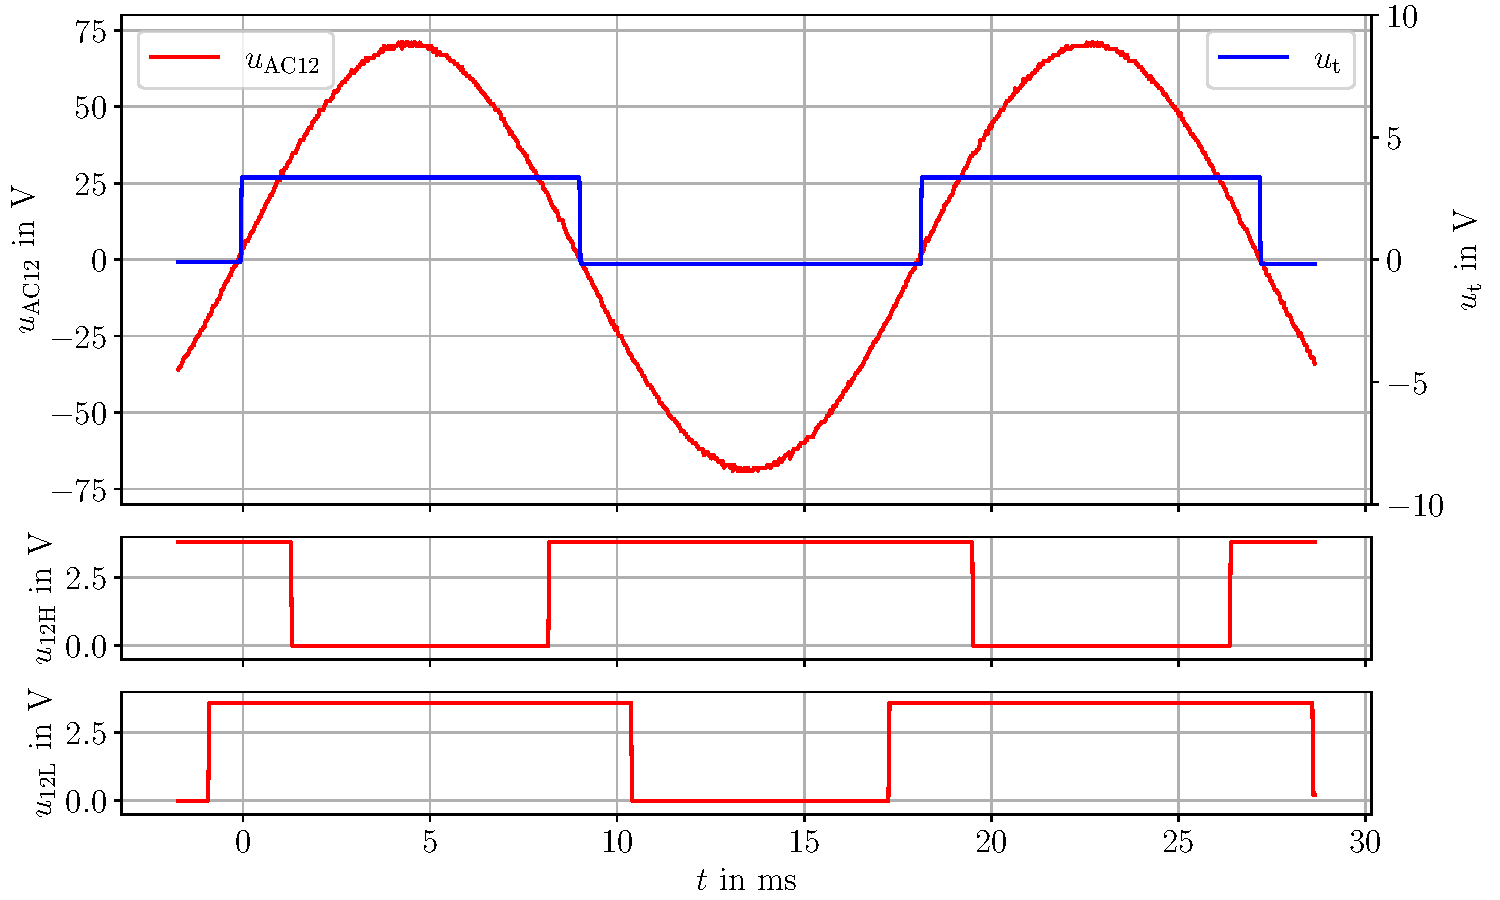
\includegraphics[width=0.95\linewidth]{IbGridSync}
    \caption{Signalverläufe der Phasenerkennungsschaltung bei $f~=~55~\text{Hz}$. Durch die Auswertung der Ausgangssignale $u_\text{12\{L,H\}}$ der Opto-Emulatoren kann der Mikrocontroller den Nulldurchgang exakt vorhersagen (siehe Testausgangssignal $u_\text{t}$).}	
    \label{fig:InGridSync}
\end{figure}


\end{document}